\documentclass[12pt]{article}
\usepackage[danish]{babel}
\usepackage{amsfonts, amssymb, mathtools, amsthm, amsmath}
\usepackage{graphicx, pgfplots}
\usepackage{url}
\usepackage[dvipsnames]{xcolor}
\usepackage{sagetex}
\usepackage{lastpage}

%loaded last
\usepackage[hidelinks]{hyperref}

\usepackage{siunitx}
  \sisetup{exponent-product = \cdot,
    output-decimal-marker = {,}}

%Giles Castelles incfig
\usepackage{import}
\usepackage{xifthen}
\usepackage{pdfpages}
\usepackage{transparent}

\newcommand{\incfig}[2][1]{%
  \def\svgwidth{#1\columnwidth}
  \import{../figures/}{#2.pdf_tex}
}

\setlength{\parindent}{0in}
\setlength{\oddsidemargin}{0in}
\setlength{\textwidth}{6.5in}
\setlength{\textheight}{8.8in}
\setlength{\topmargin}{0in}
\setlength{\headheight}{18pt}

\usepackage{fancyhdr}
\pagestyle{fancy}

\fancyhead{}
\fancyfoot{}
\fancyfoot[R]{\thepage}
\fancyhead[C]{\leftmark}

\pgfplotsset{compat=newest}

\pgfplotsset{every axis/.append style={
  axis x line=middle,    % put the x axis in the middle
  axis y line=middle,    % put the y axis in the middle
  axis line style={<->,color=black}, % arrows on the axis
}}

\usepackage{thmtools}
\usepackage{tcolorbox}
  \tcbuselibrary{skins, breakable}
  \tcbset{
    space to upper=1em,
    space to lower=1em,
  }

\theoremstyle{definition}

\newtcolorbox[auto counter]{definition}[1][]{%
  breakable,
  colframe=ForestGreen,  %frame color
  colback=ForestGreen!5, %background color
  colbacktitle=ForestGreen!25, %background color for title
  coltitle=ForestGreen!70!black,  %title color
  fonttitle=\bfseries\sffamily, %title font
  left=1em,              %space on left side in box,
  enhanced,              %more options
  frame hidden,          %hide frame
  borderline west={2pt}{0pt}{ForestGreen},  %display left line
  title=Definition \thetcbcounter: #1,
}

\newtcolorbox{greenline}{%
  breakable,
  colframe=ForestGreen,  %frame color
  colback=white,          %remove background color
  left=1em,              %space on left side in box
  enhanced,              %more options
  frame hidden,          %hide frame
  borderline west={2pt}{0pt}{ForestGreen},  %display left line
}

\newtcolorbox[auto counter, number within=section]{eks}[1][]{%
  brekable,
  colframe=NavyBlue,  %frame color
  colback=NavyBlue!5, %background color
  colbacktitle=NavyBlue!25,    %background color for title
  coltitle=NavyBlue!70!black,  %title color
  fonttitle=\bfseries\sffamily, %title font
  left=1em,            %space on left side in box,
  enhanced,            %more options
  frame hidden,        %hide frame
  borderline west={2pt}{0pt}{NavyBlue},  %display left line
  title=Eksempel \thetcbcounter: #1
}

\newtcolorbox{blueline}{%
  breakable,
  colframe=NavyBlue,     %frame color
  colback=white,         %remove background
  left=1em,              %space on left side in box,
  enhanced,              %more options
  frame hidden,          %hide frame
  borderline west={2pt}{0pt}{NavyBlue},  %display left line
}

\newtcolorbox{teo}[1][]{%
  breakable,
  colframe=RawSienna,  %frame color
  colback=RawSienna!5, %background color
  colbacktitle=RawSienna!25,    %background color for title
  coltitle=RawSienna!70!black,  %title color
  fonttitle=\bfseries\sffamily, %title font
  left=1em,              %space on left side in box,
  enhanced,              %more options
  frame hidden,          %hide frame
  borderline west={2pt}{0pt}{RawSienna},  %display left line
  title=Teori: #1,
}

\newtcolorbox[auto counter, number within=section]{sæt}[1][]{%
  breakable,
  colframe=RawSienna,  %frame color
  colback=RawSienna!5, %background color
  colbacktitle=RawSienna!25,    %background color for title
  coltitle=RawSienna!70!black,  %title color
  fonttitle=\bfseries\sffamily, %title font
  left=1em,              %space on left side in box,
  enhanced,              %more options
  frame hidden,          %hide frame
  borderline west={2pt}{0pt}{RawSienna},  %display left line
  title=Sætning \thetcbcounter: #1,
  before lower={\textbf{Bevis:}\par\vspace{0.5em}},
  colbacklower=RawSienna!25,
}

\newtcolorbox{redline}{%
  breakable,
  colframe=RawSienna,  %frame color
  colback=white,       %Remove background color
  left=1em,            %space on left side in box,
  enhanced,            %more options
  frame hidden,        %hide frame
  borderline west={2pt}{0pt}{RawSienna},  %display left line
}

\newtcolorbox{for}[1][]{%
  breakable,
  colframe=NavyBlue,  %frame color
  colback=NavyBlue!5, %background color
  colbacktitle=NavyBlue!25,    %background color for title
  coltitle=NavyBlue!70!black,  %title color
  fonttitle=\bfseries\sffamily, %title font
  left=1em,              %space on left side in box,
  enhanced,              %more options
  frame hidden,          %hide frame
  borderline west={2pt}{0pt}{NavyBlue},  %display left line
  title=Forklaring #1,
}

\newtcolorbox{bem}{%
  breakable,
  colframe=NavyBlue,  %frame color
  colback=NavyBlue!5, %background color
  colbacktitle=NavyBlue!25,    %background color for title
  coltitle=NavyBlue!70!black,  %title color
  fonttitle=\bfseries\sffamily, %title font
  left=1em,              %space on left side in box,
  enhanced,              %more options
  frame hidden,          %hide frame
  borderline west={2pt}{0pt}{NavyBlue},  %display left line
  title=Bemærkning:,
}

\makeatother
\def\@lecture{}%
\newcommand{\lecture}[3]{
  \ifthenelse{\isempty{#3}}{%
    \def\@lecture{Lecture #1}%
  }{%
    \def\@lecture{Lecture #1: #3}%
  }%
  \subsection*{\makebox[\textwidth][l]{\@lecture \hfill \normalfont\small\textsf{#2}}}
}

\makeatletter

\newcommand{\opgave}[1]{%
 \def\@opgave{#1}%
 \subsection*{Opgave #1}
}

\makeatother

%Format lim the same way in intext and in display
\let\svlim\lim\def\lim{\svlim\limits}

% horizontal rule
\newcommand\hr{
\noindent\rule[0.5ex]{\linewidth}{0.5pt}
}

\title{TØ-opgaver uge 11}
\author{Noah Rahbek Bigum Hansen}
\date{12. November 2024}

\begin{document}

\maketitle

\section*{Opg. 1}
Vi skal differentiere funktionen $f(x)$, givet ved
\[ 
f(x) = \sin \left( e^{3x} \right)
.\]

\section*{1.}
Differentier $f$ ved hjælp af Python.
\bigbreak
Følgende prompt er givet til Anaconda Assistant 4.0.39: 

\begin{blueline}
  python code for differentiating $sin(e^{3x})$ (using no context from Notebook).
\end{blueline}

Anaconda Assistant gav da følgende python-kode:
\begin{verbatim}
  import sympy as sp

  # Define the variable and the function
  x = sp.symbols('x')
  function = sp.sin(sp.exp(3 * x))

  # Differentiate the function
  derivative = sp.diff(function, x)
  derivative
\end{verbatim}

Hvilket giver følgende resultat når koden køres
\[ 
3e^{3x}\cos \left( e^{3x} \right)
.\]


\section*{2.}
Differentier $f$ i hånden ved hjælp af matematik. Får du det samme resultat i begge tilfælde?
\bigbreak
Kædereglen siger at
\[ 
y' = f'(g(x)) \cdot g'(x) 
.\]
I tilfældet ovenfor sætter vi
\[ 
f(u) = \sin(u), \text{ hvor } u = e^{3x}
.\]
Vi får dermed
\[ 
y' = 3e^{3x}\cos(3^{3x})
.\]
Dette er altså det samme resultat som blev fundet vha. Python.



\section*{Opg. 2}
I denne opgave skal vi beregne integralet
\[ 
\int_{0}^{1} e^{-x^2} \, \mathrm{d}x 
\]
ved hjælp af Python. Det kan bemærkes, at integralet ikke kan udregnes ved hjælp af elementære funktioner.
\bigbreak
Følgende prompt er givet til Anaconda Assistant 4.0.39: 

\begin{blueline}
  python code for integrating $e^{-x^2}$ from 0 to 1
\end{blueline}

Anaconda Assistant gav da følgende python-kode:
\begin{verbatim}
  import numpy as np
  from scipy.integrate import quad

  # Define the function to integrate
  def integrand(x):
    return np.exp(-x**2)

  # Perform the integration from 0 to 1
  result, error = quad(integrand, 0, 1)
\end{verbatim}

Hvilket giver følgende resultat når koden køres
\[ 
  \num{0.7468241328124271} 
.\]


\section*{Opg. 3}
I denne opgave skal vi beregne integralet
\begin{equation} \label{eq:1}
  \int_{0}^{1} \int_{0}^{y} x^2y^2 \, \mathrm{d}x \, \mathrm{d}y
\end{equation}

\subsection*{1.}
Beregn integralet (\ref{eq:1}) ved hjælp af Python.

Følgende prompt er givet til Anaconda Assistant 4.0.39: 

\begin{blueline}
  python code for calculating the integral of the integral of $x^2y^2 \mathrm{d}x \mathrm{d}y$ from 0 to $y$ from 0 to 1
\end{blueline}

Anaconda Assistant gav da følgende python-kode:
\begin{verbatim}
  import sympy as sp

  # Define the variables
  x, y = sp.symbols('x y')

  # Define the function
  function = x**2 * y**2

  # Perform the first integral with respect to x from 0 to y
  inner_integral = sp.integrate(function, (x, 0, y))

  # Now perform the second integral with respect to y from 0 to 1
  result = sp.integrate(inner_integral, (y, 0, 1))

  result
\end{verbatim}

Hvilket giver følgende resultat når koden køres
\[ 
  \frac{1}{18}
.\]

\subsection*{2.}
Beregn integralet (\ref{eq:1}) i hånden ved hjælp af matematik. Får du det samme resultat i begge tilfælde?
\bigbreak
Først beregnes det inderste integrale som
\begin{align*}
  y^2 \int_{0}^{y} x^2 \, \mathrm{d}x &= \left[ \frac{1}{3}x^{3} \right]_0^{y} \\
  &= \frac{1}{3}y^{3} \\
.\end{align*}
Og det yderste integrale som
\begin{align*}
  \frac{1}{3} \int_{0}^{1} y^{5} \, \mathrm{d}y &= \left[ \frac{1}{6}y^{6} \right]_0^1  \\
  &= \frac{1}{3\cdot6} \\
  &= \frac{1}{18}
.\end{align*}
Hvilket altså er det samme resultat som Python-koden gav.


\section*{Opg. 4}
Betragt differentialligningen
\begin{equation} \label{eq:2}
  y' = y^2 + 4
\end{equation}

\subsection*{1.}
Er differentialligningen (\ref{eq:2}) lineær?
\bigbreak
Nej, idet der indgår et $y^2$-led er differentialligningen ikke en linearkombination af $y$ og $y$'s afledede

\subsection*{2.}
Benyt Python til at løse ligningen (eksakt).
\bigbreak
Følgende prompt er givet til Anaconda Assistant 4.0.39: 

\begin{blueline}
  python code for solving the differential equation $y' = y^2 + 4$ 
\end{blueline}

Anaconda Assistant gav da følgende python-kode:
\begin{verbatim}
  import sympy as sp

  # Define the variables
  y = sp.Function('y')
  x = sp.symbols('x')

  # Define the differential equation
  differential_eq = sp.Eq(y(x).diff(x), y(x)**2 + 4)

  # Solve the differential equation
  solution = sp.dsolve(differential_eq, y(x))

  solution
\end{verbatim}

Hvilket giver følgende resultat når koden køres
\[ 
  y(x) = -2 \tan(C_1 - 2x)
.\]



\subsection*{3.}
Plot løsningen til (\ref{eq:2}).
\bigbreak
Følgende prompt er givet til ChatGPT 4o: 

\begin{blueline}
  python code for solving the differential equation $y' = y^2 + 4$ 
\end{blueline}

Anaconda Assistant gav da følgende python-kode:
\begin{verbatim}
  import numpy as np
  import matplotlib.pyplot as plt
  from scipy.integrate import odeint

  # Define the differential equation with correct arguments
  def dydx(y, x):
      return y**2 + 4

  # Set the range of x values
  x = np.linspace(0, 10, 100)

  # Initial condition
  y0 = 0.0

  # Solve the differential equation using odeint
  y = odeint(dydx, y0, x, tfirst=True)

  # Plot the solution
  plt.plot(x, y[:, 0], label="y'(x) = y^2 + 4")
  plt.xlabel('x')
  plt.ylabel('y')
  plt.title("Solution to the differential equation y' = y^2 + 4")
  plt.legend()
  plt.grid(True)
  plt.show()
\end{verbatim}

Hvilket giver følgende resultat når koden køres

\begin{figure} [ht]
  \centering
  \caption{Resultatet af Python-koden}
  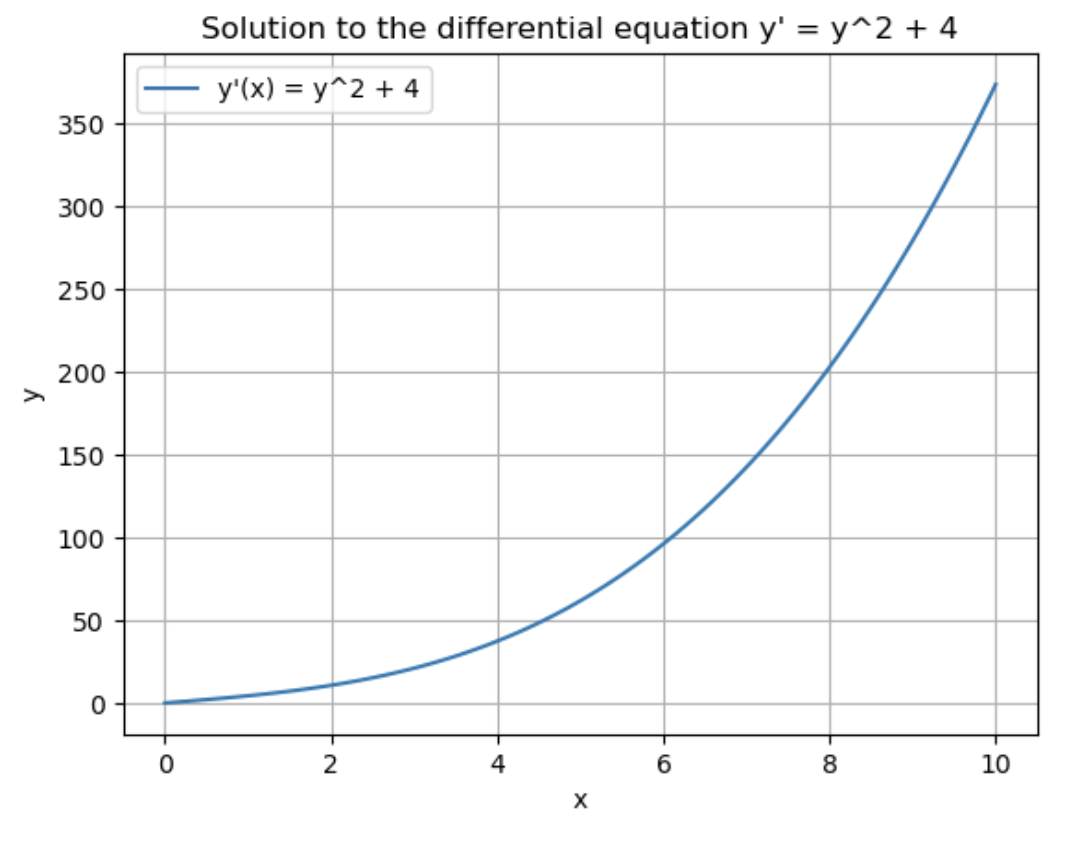
\includegraphics[width=0.8\linewidth]{../figures/TO_11_1.png}
  \label{fig:TO_11_1}
\end{figure}

\section*{Opg. 5}
Lad $f(x,y)$ betegne funktionen
\[ 
f(x,y) = x^3y - y^3x
.\]
Maksimer funktion $f(x,y)$ over området $0 \leq x \leq 1$ og $0 \leq y \leq 1$ ved hjælp af Python.

Ufordring (lidt svært): Overvej om du kan løse denne opgave i hånden vha. matematik
\bigbreak
Følgende prompt er givet til Anaconda Assistant 4.0.39: 

\begin{blueline}
  Write some python code that maximizes $x^3y - y^3x$ over the interval 0 <= x <= 1 and 0 <= y <= 1
\end{blueline}

Anaconda Assistant gav da følgende python-kode:
\begin{verbatim}
  import numpy as np
  from scipy.optimize import minimize

  # Define the function to maximize
  def objective(vars):
    x, y = vars
    return -(x**3 * y - y**3 * x)  # Negate to convert maximization to minimization

  # Define the bounds for x and y
  bounds = [(0, 1), (0, 1)]

  # Initial guess
  initial_guess = [0.5, 0.5]

  # Perform the optimization
  result = minimize(objective, initial_guess, bounds=bounds)

  # Extract the optimal values
  optimal_x, optimal_y = result.x
  max_value = -result.fun  # Negate again to get the maximum value

  optimal_x, optimal_y, max_value
\end{verbatim}

Hvilket giver følgende resultat når koden køres
\[ 
  (1.0, 0.5773501788044133, 0.38490017945973637)
.\]
I koden kan det aflæses at dette skal tolkes som at punktet hvor funktionen er maksimeret er $(1,0; 0,577)$, hvor funktionsværdien er $0,385$.


\end{document}
